\chapter{Mesh Generation}
%

\begin{figure}[ht]
\centering
\subfigure[]{%
		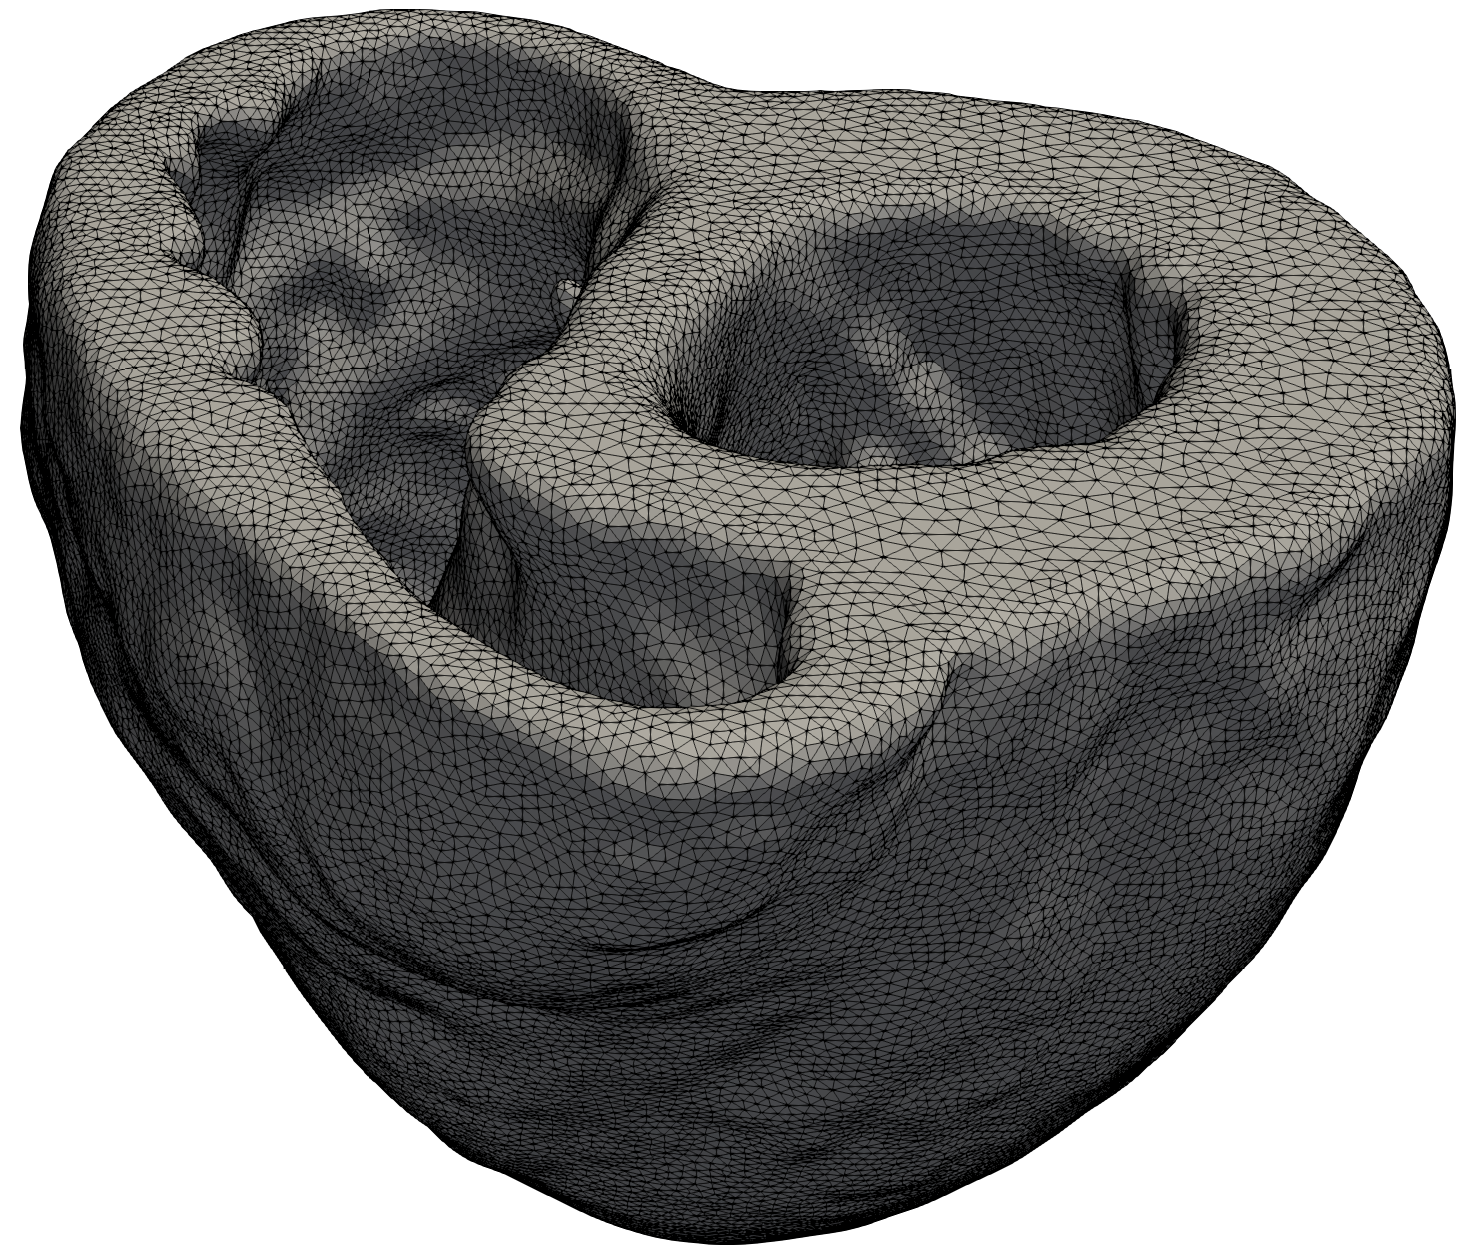
\includegraphics[scale=0.14]{media/4-cardioid/0-ventriclesurf.png}
\label{fig:tet1}}
\subfigure[]{%
		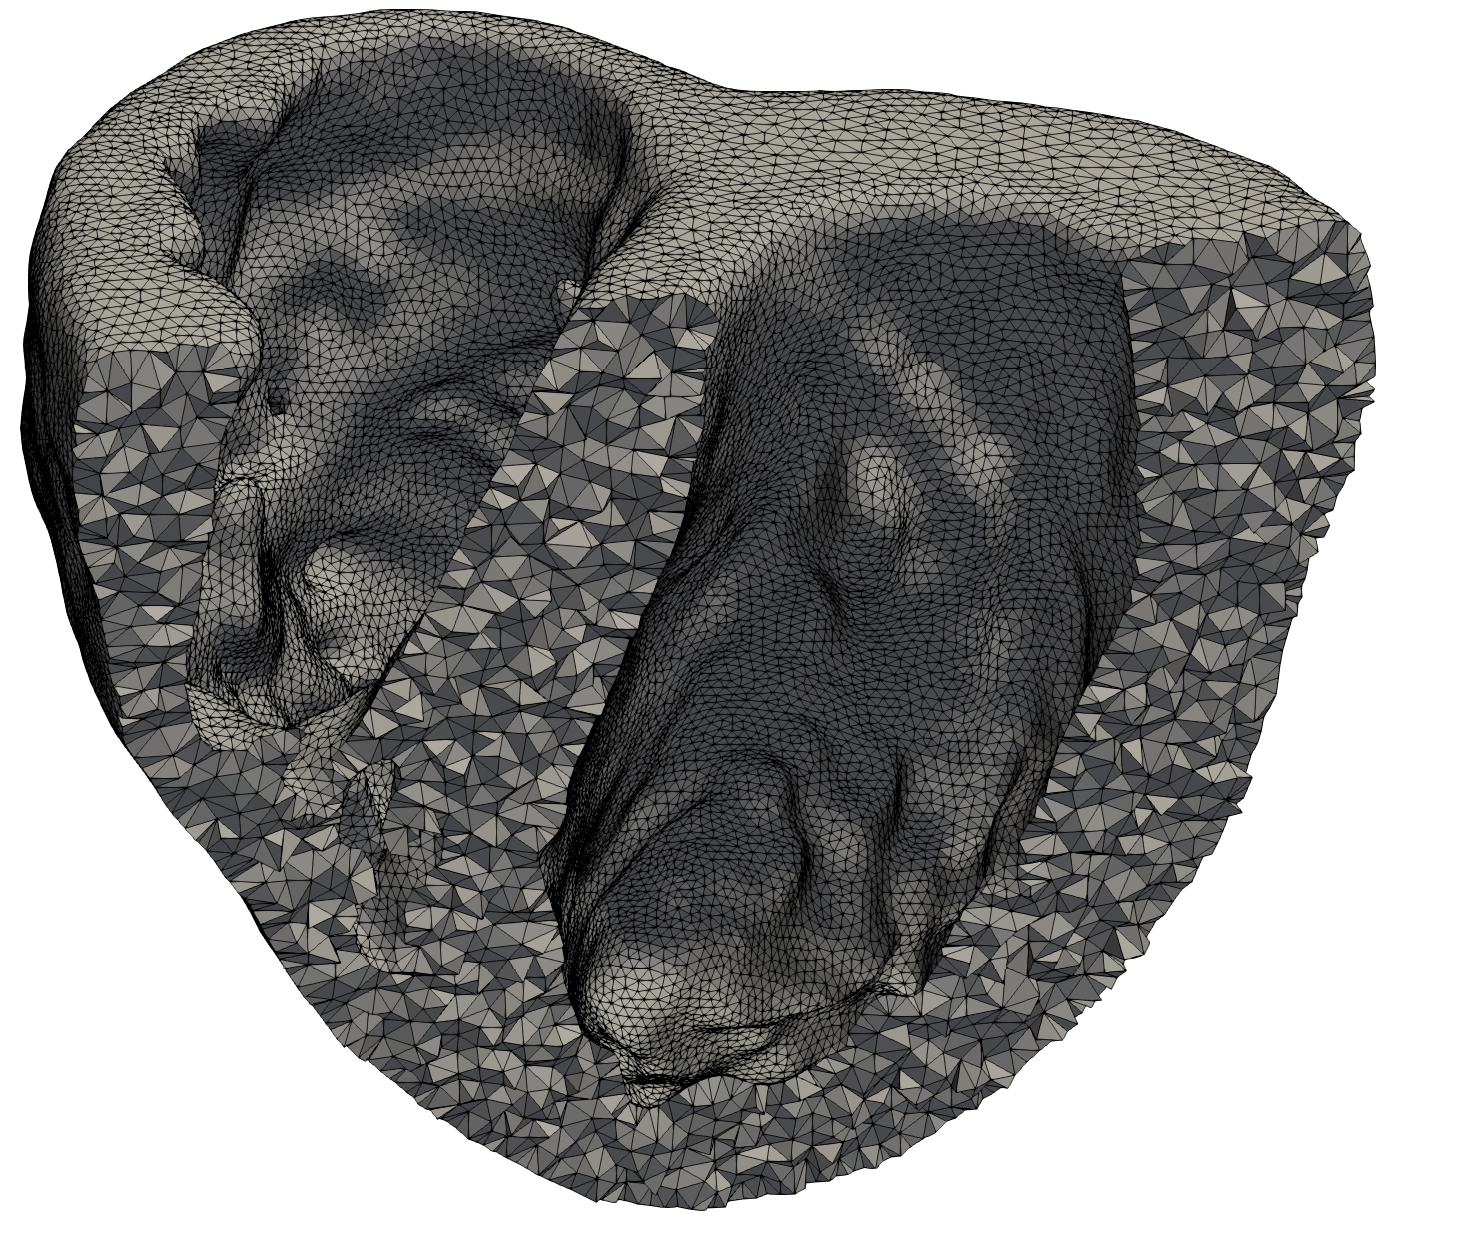
\includegraphics[scale=0.14]{media/4-cardioid/1-tet.png}
\label{fig:tet2}}
%
\caption{Bi-ventricular mesh: (a) surface mesh, and (b) clipped view of quadratic tetrahedral mesh used in Cardioid simulations}
\label{fig:tetmesh}
\end{figure}

\begin{figure}[ht]
\centering
\subfigure[]{%
		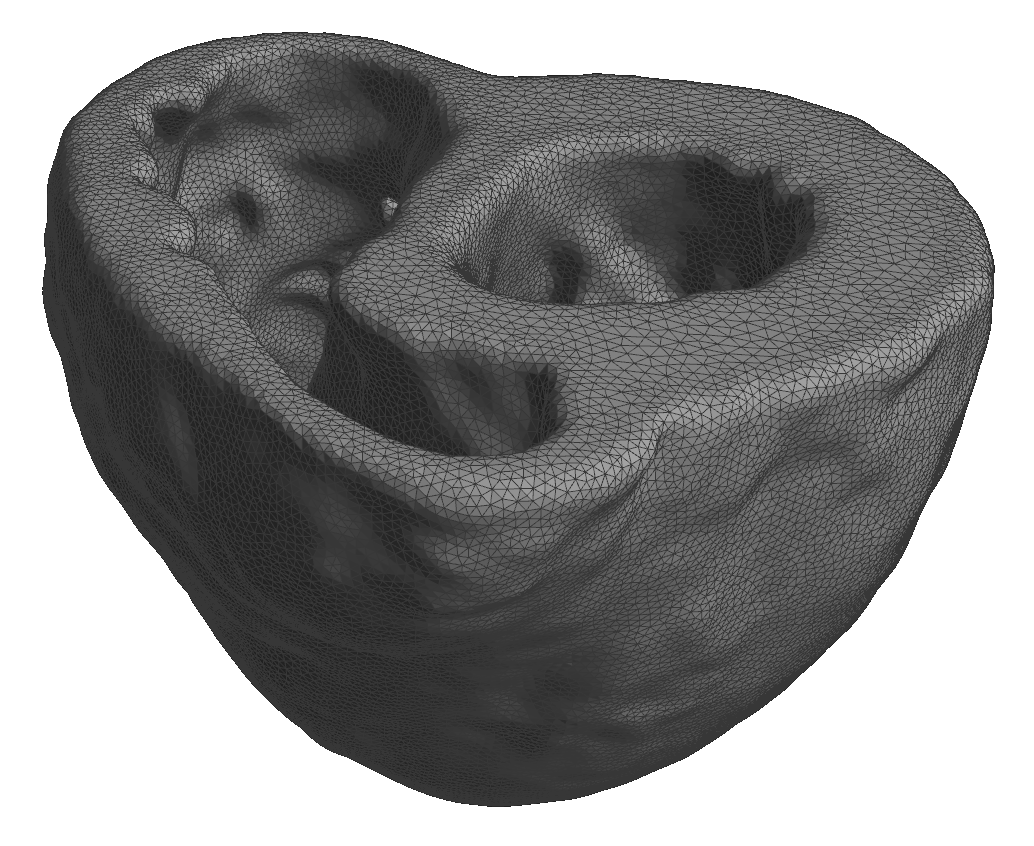
\includegraphics[scale=0.2]{media/3-celeris/1-brep.png}
\label{fig:cel1}}		
\subfigure[]{%
		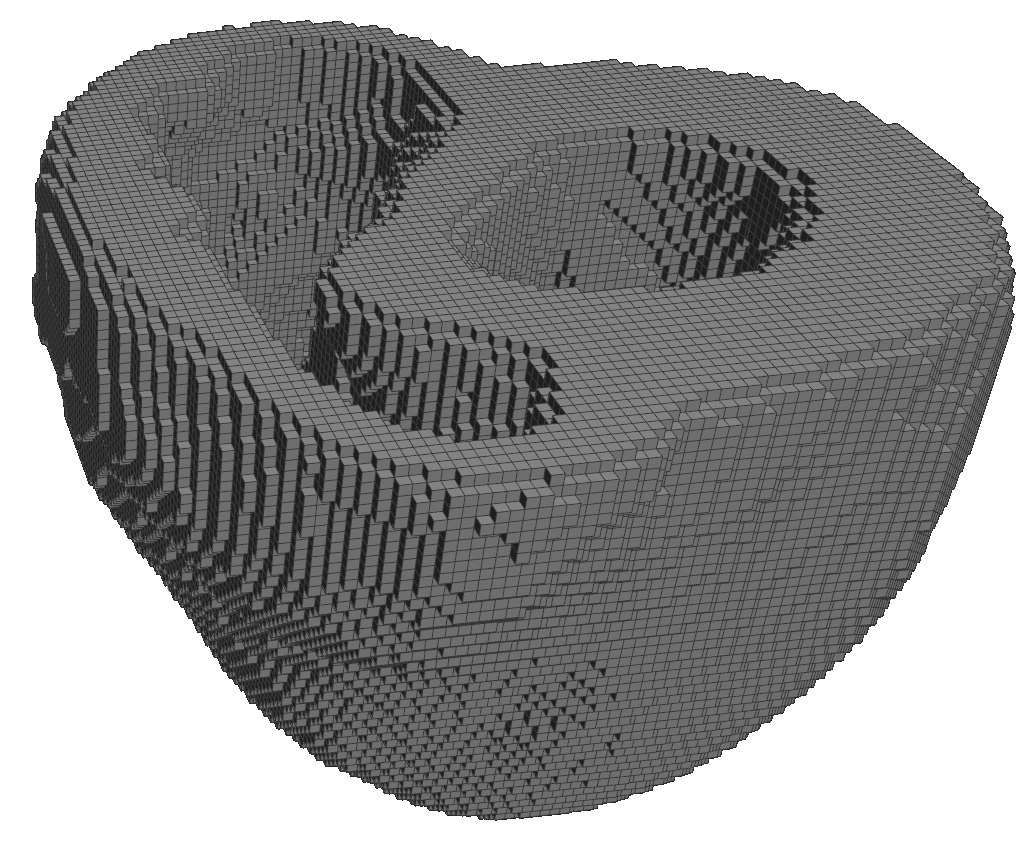
\includegraphics[scale=0.2]{media/3-celeris/2-hex.png}
\label{fig:cel2}}		
\subfigure[]{%
		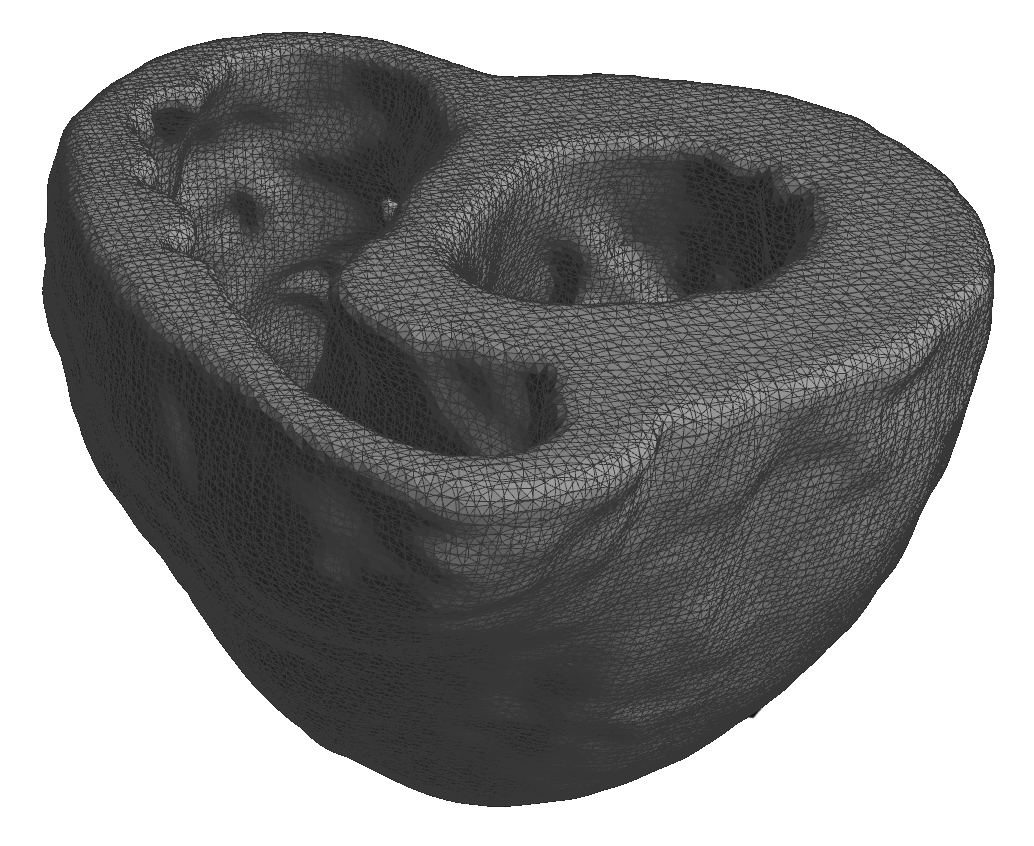
\includegraphics[scale=0.2]{media/3-celeris/3-pmesh.png}
\label{fig:cel3}}		
\subfigure[]{%
		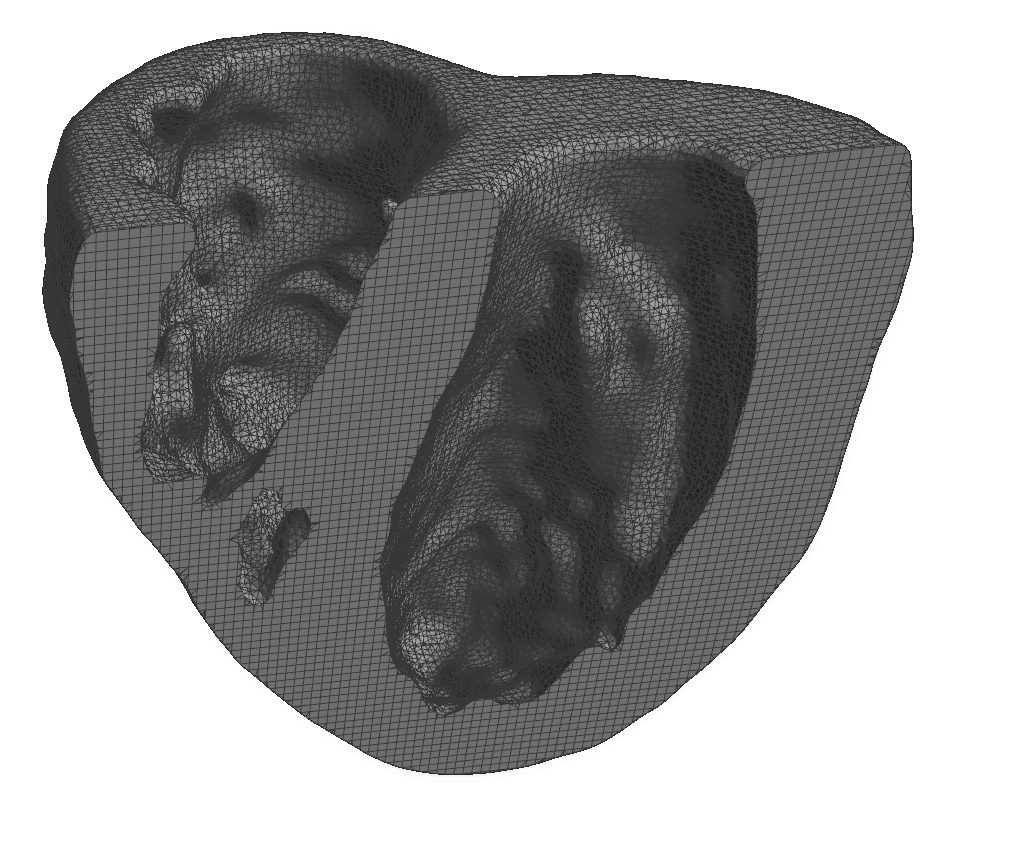
\includegraphics[scale=0.2]{media/3-celeris/4-clip.png}
\label{fig:cel4}}	
\subfigure[]{%
		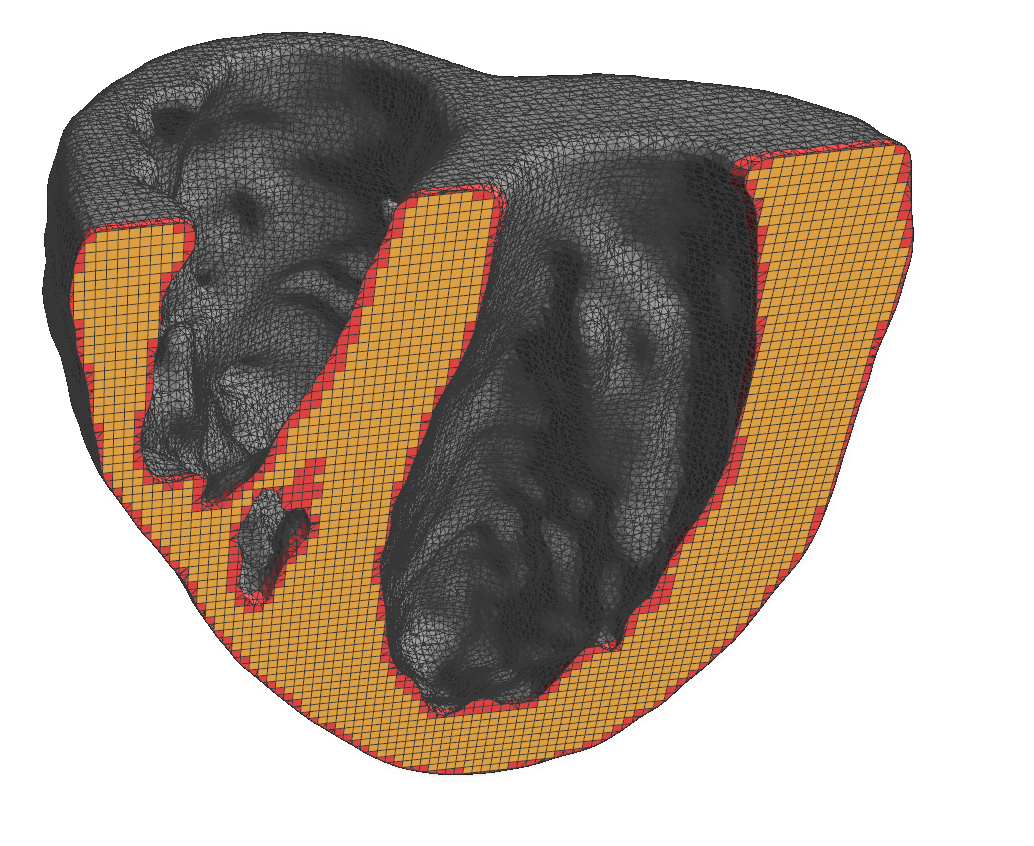
\includegraphics[scale=0.2]{media/3-celeris/5-color.png}
\label{fig:cel5}}			

\caption{Generation of polyhedral mesh: (a) input surface mesh, (b) bounding hex mesh,  (c) resulting polyhedral mesh, (d) clipped mesh, and (e) highlight of elements with cuboidal vs. general polyhedral shape.}
\label{fig:cel}
\end{figure}

\begin{figure}[ht]
\centering
\subfigure[]{%
		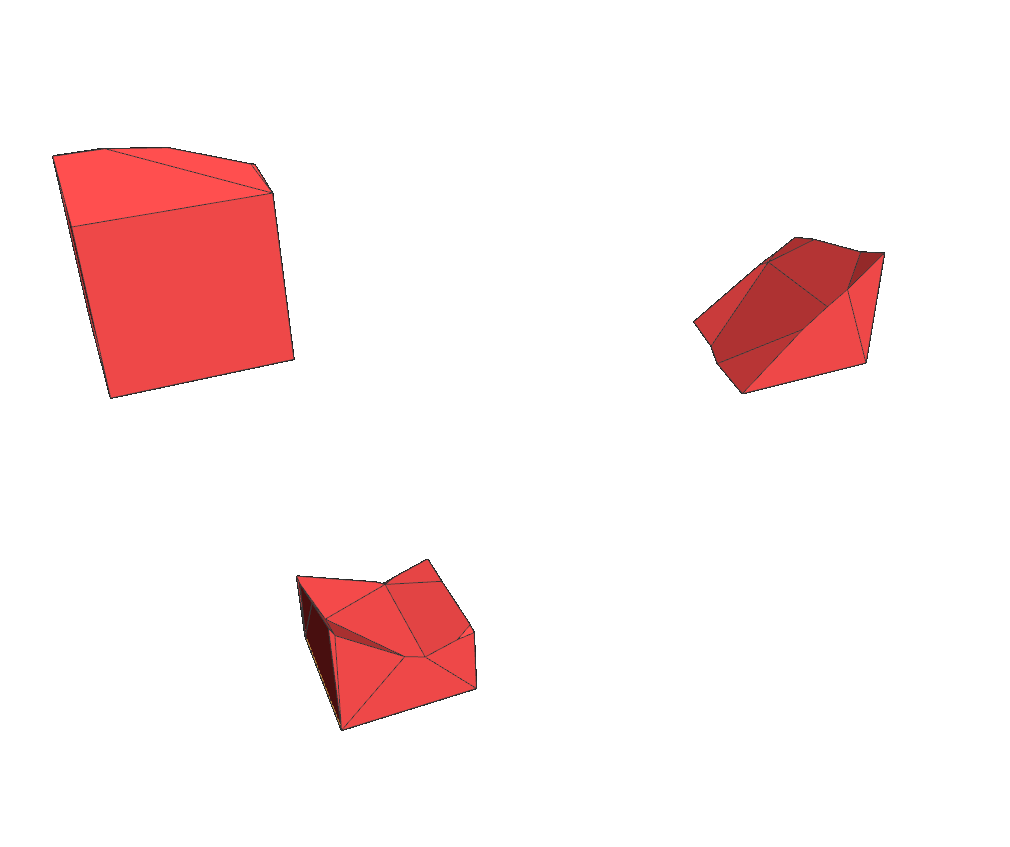
\includegraphics[scale=0.125]{media/3-celeris/zoom/zoom1.png}
\label{fig:zoom1}}		
\subfigure[]{%
		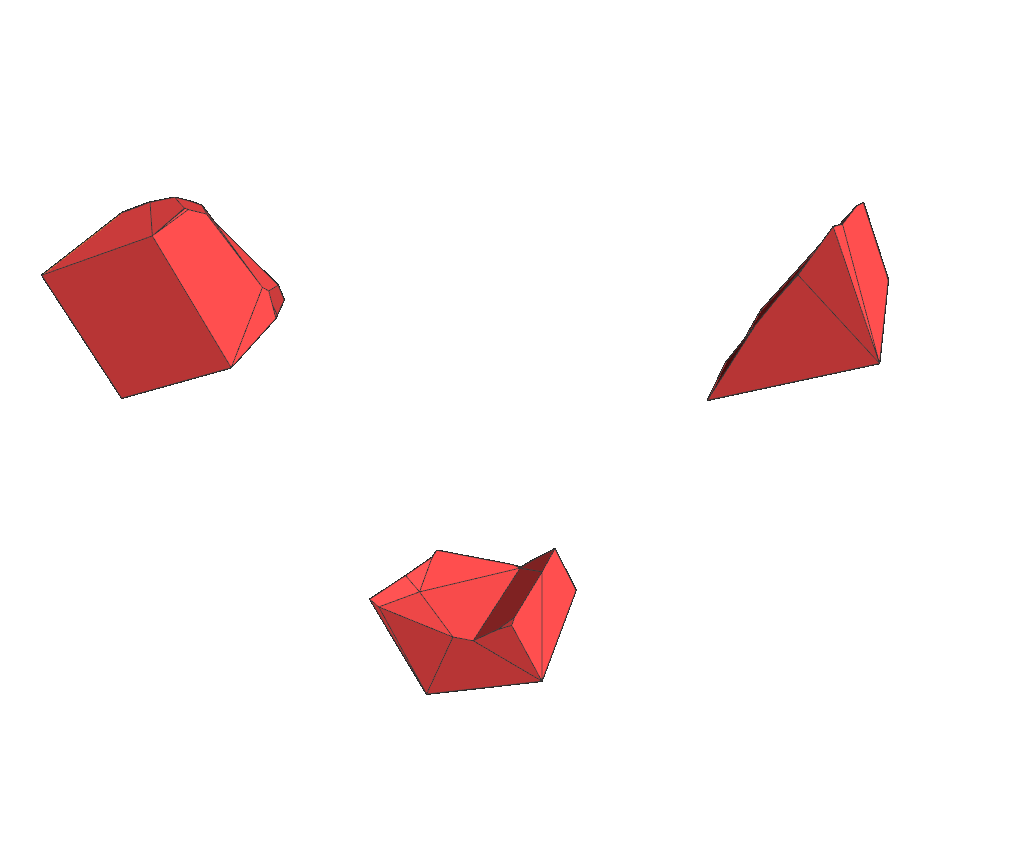
\includegraphics[scale=0.125]{media/3-celeris/zoom/zoom2.png}
\label{fig:zoom2}}		
\subfigure[]{%
		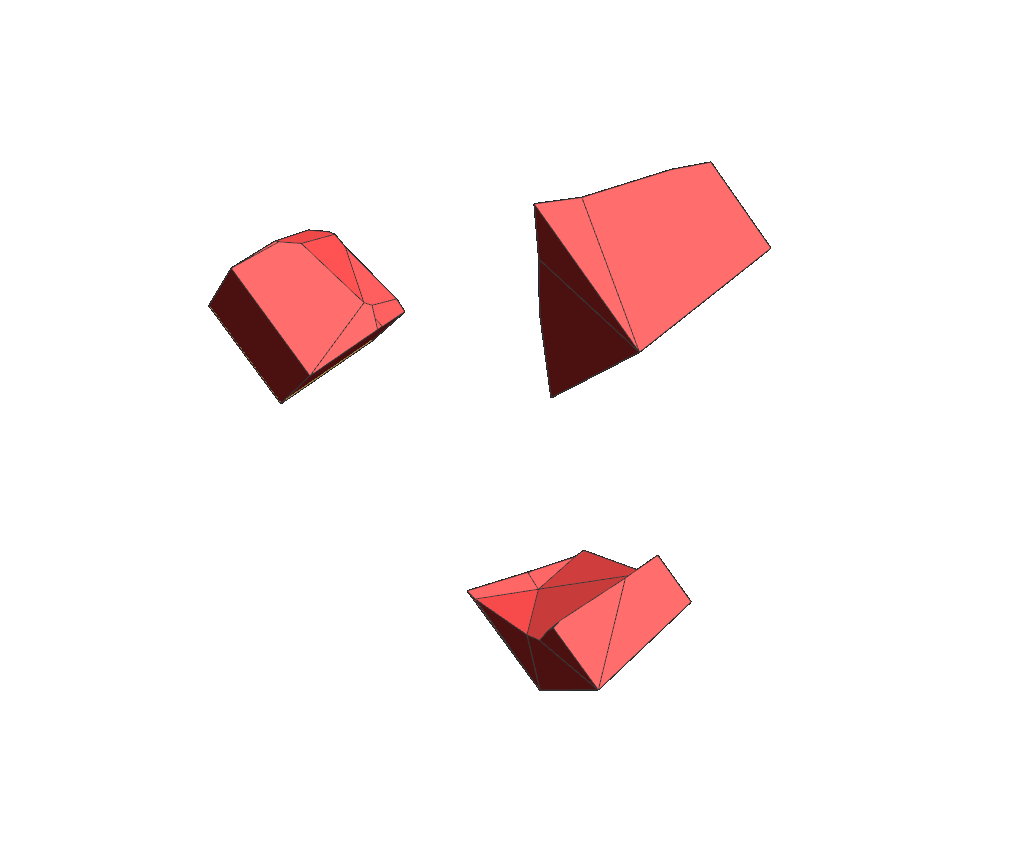
\includegraphics[scale=0.125]{media/3-celeris/zoom/zoom3.png}
\label{fig:zoom3}}		
\subfigure[]{%
		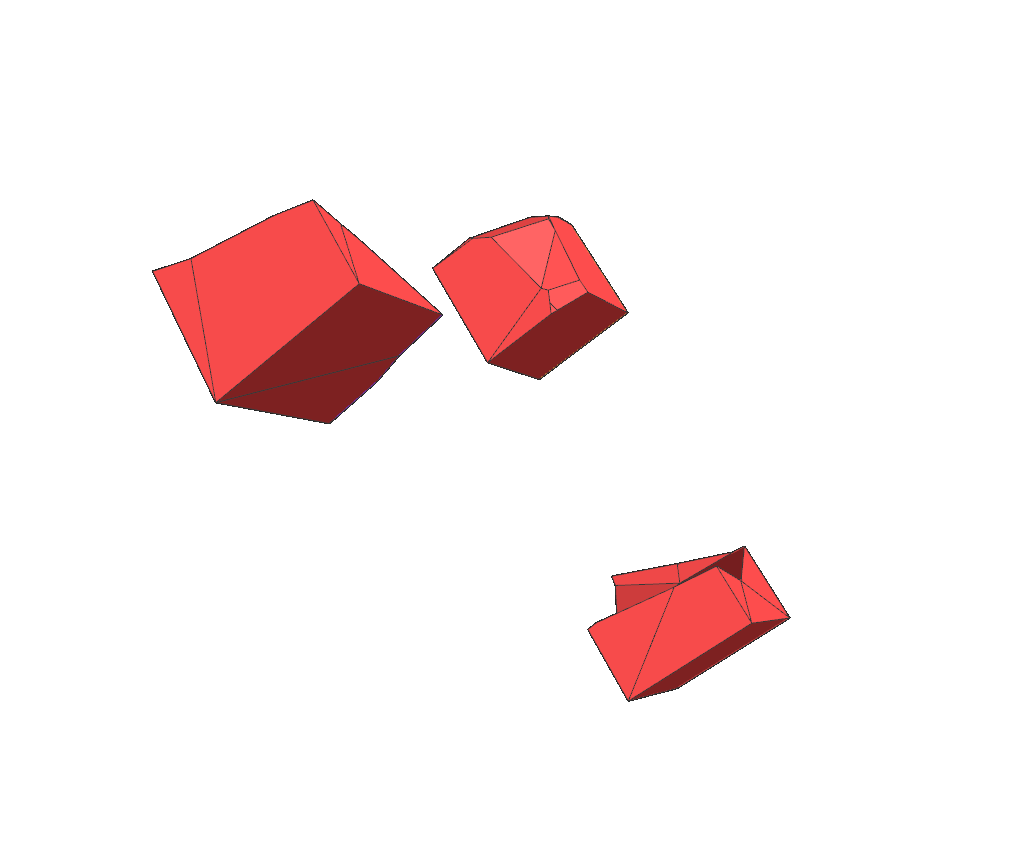
\includegraphics[scale=0.125]{media/3-celeris/zoom/zoom4.png}
\label{fig:zoom4}}	
\subfigure[]{%
		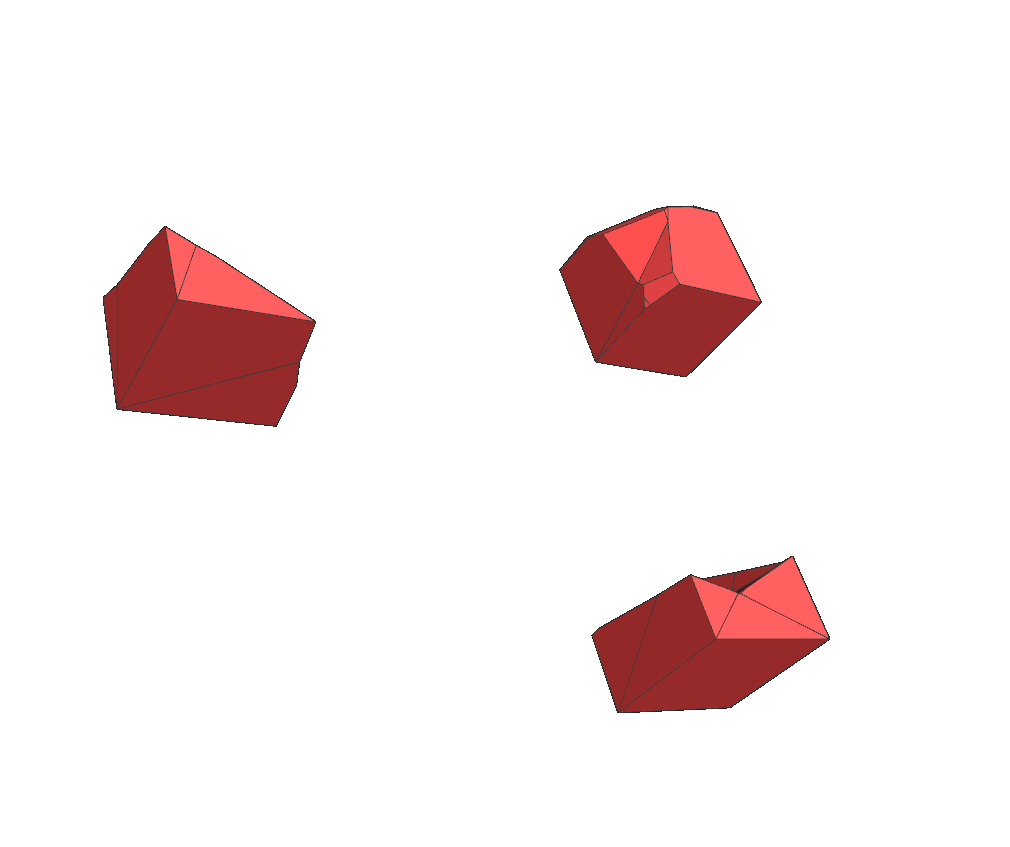
\includegraphics[scale=0.125]{media/3-celeris/zoom/zoom5.png}
\label{fig:zoom5}}		
\subfigure[]{%
		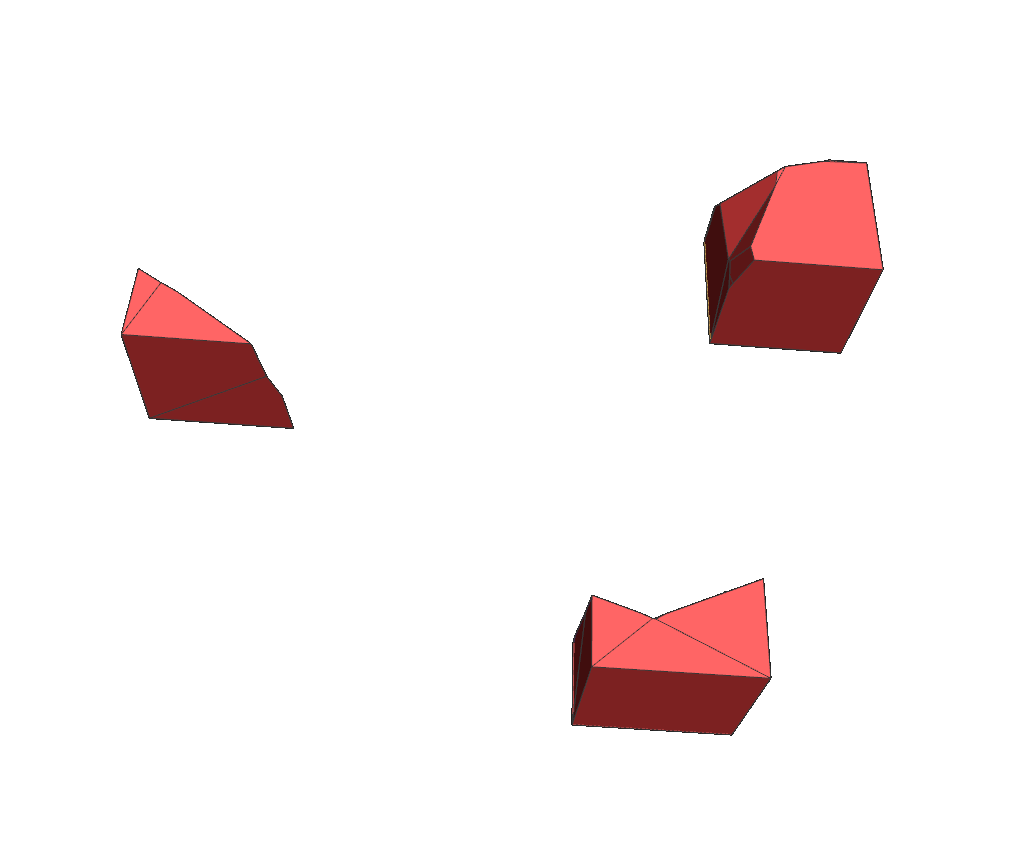
\includegraphics[scale=0.125]{media/3-celeris/zoom/zoom6.png}
\label{fig:zoom6}}	

\caption{Three example arbitrary polyhedral elements presented at different angles}
\label{fig:zoom}
\end{figure}

\begin{figure}[ht]
\centering
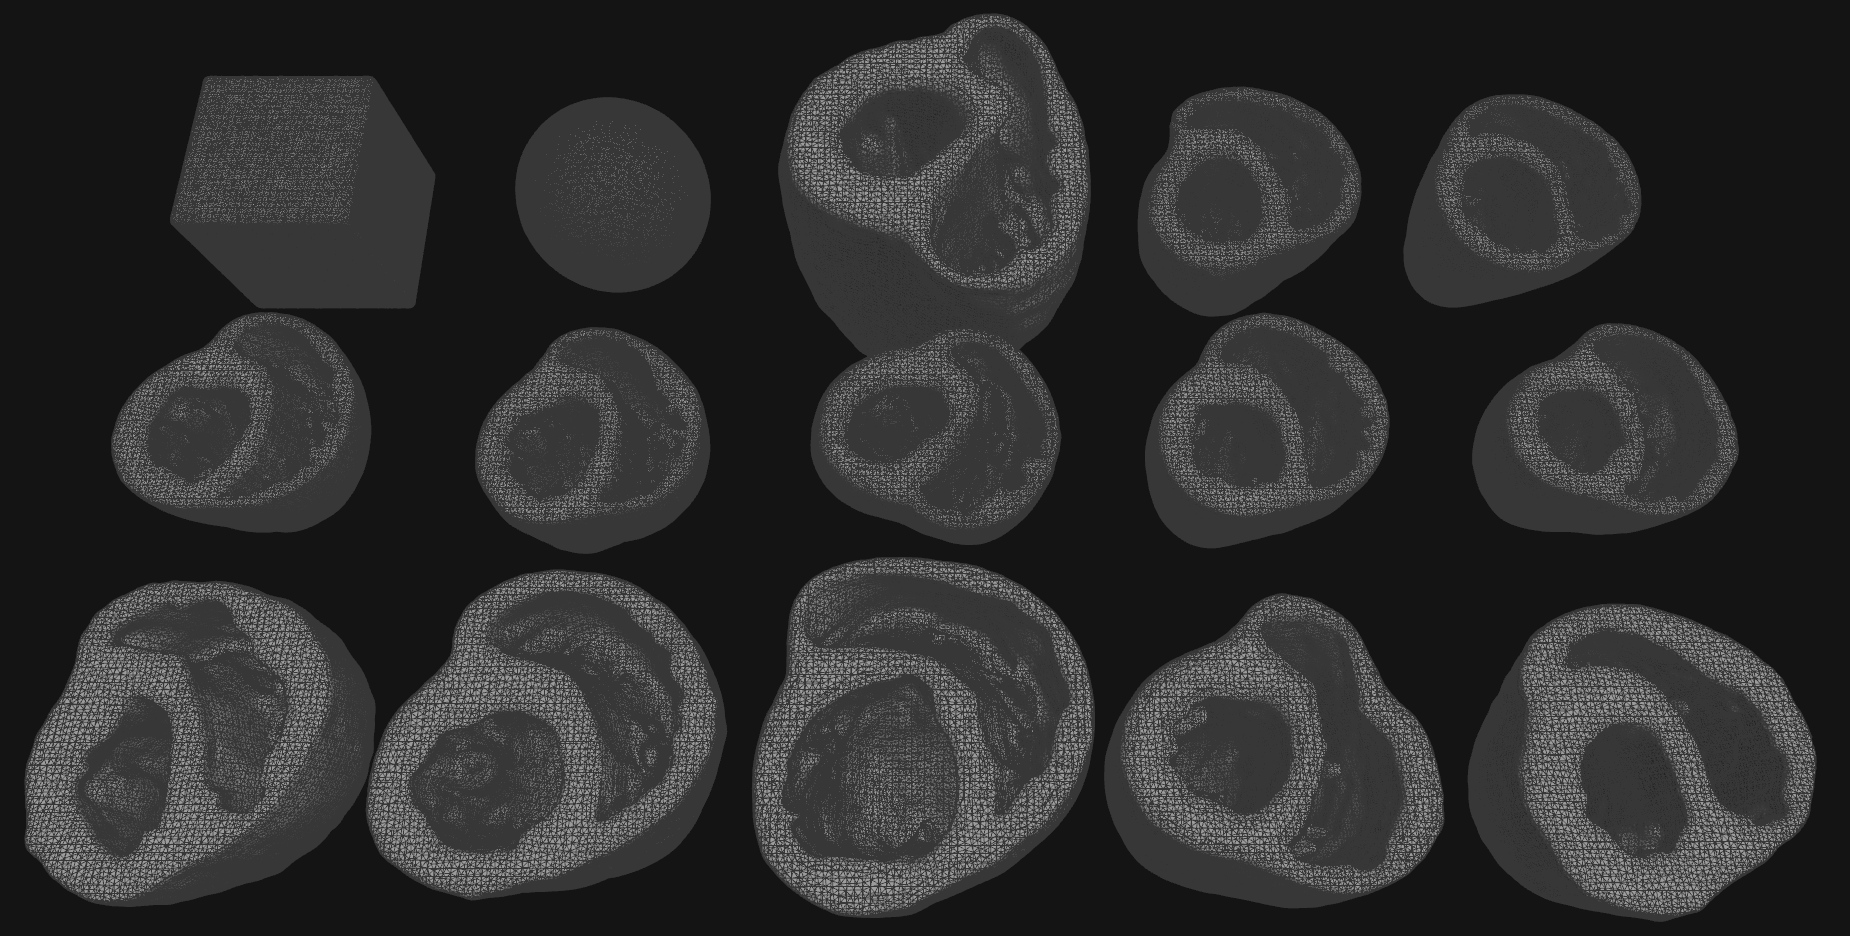
\includegraphics[width=1.0\textwidth]{media/3-celeris/7-suite.png}
\caption{Suite of polyhedral finite element meshes generated from image data \vspace{1cm}}
\label{fig:celsuite}
\end{figure}



%%%%%%%%%%%%%%%%%%%%%%%%%%%%%%%%%%%%%%%%%%%%%%%
%%%%%%%%%%%%%%%%%%%%%%%%%%%%%%%%%%%%%%%%%%%%%%%
\section{Review of Mesh Generation Techniques}
\label{Review of Mesh Generation Techniques}

Don't forget PhDResearch/doc/vorrecon \\

Hex meshing:
sweep mesh
thin sweep
multizone

Universal meshes for smooth surfaces with no boundary in three dimensions \\

Search Voronoi meshing from medical imaging. Or from segmented medical imaging

vmtk: http://www.vmtk.org/tutorials/ \\

http://www.robertschneiders.de/meshgeneration/software.html \\

$http://homepage.usask.ca/~ijm451/finite/fe_resources/mesh.html$ \\

- simpleware webinar \\

- downsampling - poisson disk sampling\\
- smooth normals\\
- filtering\\

- watertight surface reconstruction\\
	- vorocrust\\
	- powercrust\\
	- ball pivoting\\
	- poisson surface reconstruction\\
	- tight cocone\\
	
- meshing from CAD\\
    - tetgen\\
    - cubit/bolt\\
    
- direct meshing\\
	- simpleware\\

- smoothing after the fact\\
	- laplacian smooth\\

mesh simplification/decimation\\
cut cell approach\\
smoothing papers\\

noisy, oversampled point cloud\\


Simpleware webinar

- simpleware does not do CAD-based modeling, goes directly to the mesh
- contact regarding technical work/papers for meshing
export as STL, mesh, or NURBS
- TWO BOTTLENECKS
  - image segmentation time
  - generating watertight and error free meshes
    - no gaps or overlaps 
    - no inverted elements 
    - no negative jacobian
- segmentation -> stl -> smoothing -> nurbs -> meshing -  cad geometry medical device -> export final model -> poor elements, gaps and overlap, non convergence, not watertight
- manual corrections of stl, curbs, meshes

- generation of watertight STL
- aspect ratio/mesh quality
- image-based meshing

- BLENDR - graphics, STL
- Rhino - STL generation, NURBS

Email Kerim, k.genc@simpleware.com

see you at WCCM
Ross Cotton’s recently published paper
Ross Cotton, r.cotton@simpleware.com

Simpleware paper:
1. marching cubes for surface mesh
2. Advancing front or Delaunay techniques for tet meshing --> produces slivers though
3. Extended EVoMacs

hex meshers:

truegrid\\
cubit

mask to mesh:
dual contouring

"state of the art" papers\\
Sculpt Sandia - grid based meshing, volume fraction \\
"Parallel hex meshing from volume fractions"\\
For each voxel, sample a bunch of points, decide if inside or outside \\
Look at neighboring cells, do least squares to approximate gradient and throw down normal \\

Netgen advancing front. Mimix hex mesher \\

Truegrid hex mesher \\
CUBIT \\
Mimix \\

automated hex meshing at uconn: http://im.engr.uconn.edu/downloads.php


SURFACE RECONSTRUCTION:
show results from Poison surf recon, powercrust, tight cocone \\

SimVascular: 2D segmentations followed by lofting



DECIMATION/SURFACE COARSENING:\\
ACVD papers
Quadric Edge-Collapse Decimation

%%%%%%%%%%%%%%%%%%%%%%%%%%%%%%%%%%%%%%%%%%%%%%%
%%%%%%%%%%%%%%%%%%%%%%%%%%%%%%%%%%%%%%%%%%%%%%%
\section{Voronoi Partitioning}
\label{Voronoi Partitioning}
Voro++

%%%%%%%%%%%%%%%%%%%%%%%%%%%%%%%%%%%%%%%%%%%%%%%
%%%%%%%%%%%%%%%%%%%%%%%%%%%%%%%%%%%%%%%%%%%%%%%
\section{Tolerance-Aware Voronoi Partitioning}
\label{Tolerance-Aware Voronoi Partitioning}
%%%%%%%%%%%%%%%%%%%%%%%%%%%%%%%%%%%%%%%%%%%%%%%
%%%%%%%%%%%%%%%%%%%%%%%%%%%%%%%%%%%%%%%%%%%%%%%
\section{Voronoi-Based Mesh Generation}
\label{Voronoi-Based Mesh Generation}
%%%%%%%%%%%%%%%%%%%%%%%%%%%%%%%%%%%%%%%%%%%%%%%
%%%%%%%%%%%%%%%%%%%%%%%%%%%%%%%%%%%%%%%%%%%%%%%
\section{Boundary Representation (B-rep) Generation}
\label{Boundary Representation (B-rep) Generation}
%%%%%%%%%%%%%%%%%%%%%%%%%%%%%%%%%%%%%%%%%%%%%%%
%%%%%%%%%%%%%%%%%%%%%%%%%%%%%%%%%%%%%%%%%%%%%%%
\section{Robust Polyhedral Mesh Generation from B-reps}
\label{Robust Polyhedral Mesh Generation from B-reps}
